\chapter{Second-Order System Identification and Analysis}\label{Lab:2}
A large majority of systems we wish to control are physical systems. These
systems are often modelled using Newton's laws
\[
\begin{aligned}
  \mathrm{mass}~\frac{\mathrm d}{\mathrm{d}t}~\mathrm{position}
    &= \sum \mathrm{natural~forces} + \mathrm{applied~force},\\
  \mathrm{inertia}~\frac{\mathrm d}{\mathrm{d}t}~\mathrm{orientation}
    &= \sum \mathrm{natural~torques} + \mathrm{applied~torque},
\end{aligned}
\]
which result in second-order differential equations. These systems --- when
they are linear --- result in second-order transfer functions from the
applied input (forces or torques) to the output (position and orientation).
In other words, if we want to know how to effectively control physical systems,
we must first understand second-order systems and their properties!

In this lab you will explore the generic characteristics of a second-order
linear system. More fundamentally, you will realize the value of learning
control theory. You will discover the limitations of proportional error
feedback control --- the most na\'ive of control laws --- when applied to
a physical system. This hopefully motivates you to explore why we consider
more complicated control strategies. A future lab expands on this
idea by exploring PID control.

\emph{A word of caution. This is the final lab where it is possible to
to find out the parameters of your system by inspecting the data file.
This, in principal, allows you to back-calculate what your procedures should
tell you. This was intentional to allow
you to check your work and ensure you understand how to perform the procedure.
However, future labs will assume you've perfected the procedure.
The parameters will be fairly well hidden like how it is sometimes in the
\texttt{\#RealWorld}. So, make sure you understand how to perform the
procedures!}

\section{Objectives}
The primary objectives of this lab are to
\begin{enumerate}[label=(\arabic*)]
  \item{
    \textbf{Learn} the characteristic properties of a second-order linear
    system.
  }
  \item{
    \textbf{Identify} the parameters of a second-order linear system.
  }
  \item{
    \textbf{Learn} how to acquire a Bode plot, the frequency response,
    and \textbf{understand} how to interpret it.
  }
  \item{
    \textbf{Explore} how a proportional control feedback affects the response
    of a second-order system.
  }
\end{enumerate}
Like Lab~\ref{Lab:1}, this is not a long lab.

\section{Experimental Procedure}
This entire lab will be done using the ``\texttt{Lab\_2.slx}'' Simulink model.
In there you will
find a number of blocks already placed for you in an open loop configuration:
\begin{itemize}
  \item{a signal generator,}
  \item{a summing junction,}
  \item{an adjustable gain block,}
  \item{a ``fill-in'' disturbance block,}
  \item{a ``plant'', the system we are going to analyze, and}
  \item{a terminator.}
\end{itemize}
This time, we will \emph{not} use the signal generator and instead leverage
the Model Linearizer App. Its usage is described in Appendix
\ref{App:Simulink:ModelLinearizer}. You may acquire the step response
using the techniques described in Lab~\ref{Lab:1} but to acquire the frequency
response you will have to use the Model Linearizer app. In future, I advise
you to use the Model Linearizer app, as it'll unify all your data collection
requirements and is far easier to use than modifying a script and turning
on/off logging. For this lab, the input signal starts off configured
as \(r\) and the output signal as \(y.\) You will have to change it later
in the lab.
%
The plant --- labelled \(P(s)\) in the Simulink diagram --- can be assumed
to be a transfer function taking the form
\[
  P(s) = \frac{K}{s^2 + a s + b},
\]
where \(a, b, K > 0.\) Equivalently, we can express \(P(s)\) in what is known
as the standard second order form
\[
  P(s) = \frac{\hat{K} \omega^2}{s^2 + 2 \zeta \omega s + \omega^2}.
\]
The primary goal of this experiment is to explore
the characteristics of your system as well as how it changes as we
affect a proportional error gain.

\subsection{Measuring the Characteristics of a Second Order System}
In Lab~\ref{Lab:1}, you learned about the DC gain, the bandwidth, and
settling time of a first-order system.
We will once gain acquire the DC gain, bandwidth and settling times
whose definition does not change when applied to a second-order system.

However, there are a few more characteristics we would like to identify.
The first notion is that of the overshoot. There are a variety of ways
to define the overshoot. For us, the following definition suffices.
%
\begin{definition}[]{Time-To-Peak and Overshoot}
  Let \(G(s)\) be a proper, stable transfer function
  that maps an input signal \(u(t)\) to an output \(y(t).\)
%
  Let \(u(t)\) be the (not necessarily unit) step function. The peak value
  of \(y(t)\) is the maximum value \(y(t)\) obtains, mathematically expressed
  by
  \[
    y_\mathrm{max} \defineas \max_{\tau \in \Real} \left| y(\tau) \right|
  \]
  and the time it obtains the peak value, known as \textbf{time-to-peak}
  is defined as
  \[
    T_\mathrm{peak} \defineas \argmax_{\tau \in \Real} \left| y(\tau) \right|.
  \]
  Then, if \(y_\mathrm{ss}\) is the steady-state value of \(y(t),\) the
  \textbf{percent overshoot} is defined as
  \[
    \%\mathrm{OS}
      \defineas
        \frac{\left| y_\mathrm{max} - y_\mathrm{ss} \right|}{y_\mathrm{ss}}.
  \]
\end{definition}
%
\begin{figure}
  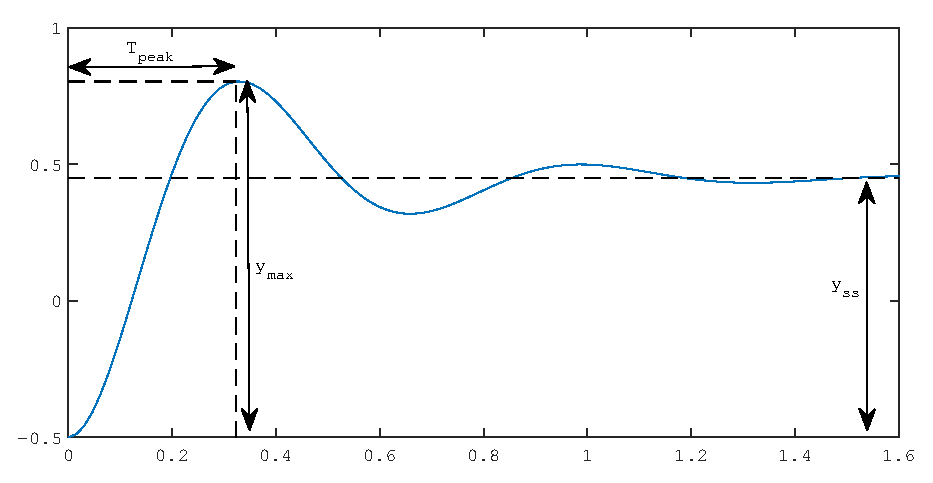
\includegraphics{images/Lab_2_Peak.eps}
  \caption[Depicting Overshoot Measurements for a Second-Order System.]{%
    The maximum peak occurs at time \(T_\mathrm{peak}\) with amplitude
    \(y_\mathrm{max}.\) The steady-state value is shown as \(y_{\mathrm{ss}}.\)
  }
  \label{fig:lab2:peak}
\end{figure}
%
Figure~\ref{fig:lab2:peak} depicts the measurements you will perform to acquire
the percent overshoot. You measure the maximum value of the output
signal and the settling value of the signal. Then you
compute the relative error between the maximum value and the settling value of
the output. The time-to-peak value is another characteristic constant we
measure.
%
\begin{procedure}[label={proc:lab2:p1}]
  In this procedure you will capture a variety of characteristics of
  your provided second-order system.
  \begin{enumerate}[label=(\arabic*)]
    \item{
      \textbf{Ensure} your system is in the open loop configuration.
    }
    \item{
      \textbf{Ensure} that you indicate the signal before the summing junction
      is an input signal (Input Perturbation) and the signal after the plant
      is indicated as an output signal (Output Measurement). Refer
      to Appendix~\ref{App:Simulink:ModelLinearizer:2} for more information
      on how to do so.
    }
    \item{
      \textbf{Open} the Model Linearizer app and \textbf{capture} a
      step response. Refer to Appendix~\ref{App:Simulink:ModelLinearizer:3}
      on how to do so.
    }
    \item{
      \textbf{Measure} and \textbf{record} the following parameters of the
      output signal:
      \begin{itemize}
        \item{
          the steady-state value \(y_{\mathrm{ss}},\)
        }
        \item{
          the time-to-peak value \(T_{\mathrm{peak}}\) and
          the peak value \(y_{\mathrm{max}},\)
        }
        \item{
          the rise time \(T_{\mathrm{rise}},\) and
        }
        \item{
          the \(2\%\) settling time \(T_{\mathrm{s}}.\)
        }
      \end{itemize}
      \label{proc:lab2:p1:4}
    }
    \item{
      \textbf{Compute} the \(\%\) overshoot of your output signal \(y(t).\)
    }
  \end{enumerate}
\end{procedure}
%
\begin{deliverable}[label={lab2:d1}]
  \textbf{Capture a figure} showing your step response \textbf{including}
  data tips at the peak value and steady-state value. Refer to
  Appendix~\ref{App:Simulink:ModelLinearizer:3} on how to do so.
\end{deliverable}

\subsection{Exploring Proportional Error Feeedback}
For this section you will explore how proportional error feedback affects
the behaviour of a second-order system. Connect your diagram so that it
looks like Figure~\ref{fig:lab2:closing-loop}.
%
\begin{figure}
  \centering
  \begin{tikzpicture}[x=1in, y=1in]
    \node [draw, block] (Controller) {\(K_p\)};
    \node [draw, block, right=0.5 of Controller] (Plant) {\(P(s)\)};
    \node [draw, summer, left=0.5 of Controller] (Sum) {};
    \node [draw, summer, right=0.5 of Plant] (DistSum) {};
    \node [above=0.5 of DistSum] (AboveDistSum) {};
    \node [below=0.5 of Sum] (BelowSum) {};

    \draw [arrow, signal]
      (AboveDistSum.base)
      --
      (DistSum.north)
      node [above right, annotate] {\(d\)};
    \draw [arrow, signal]
      (Controller.east) -- (Plant.west)
      node [below left, annotate] {\(u\)};
    \draw [arrow, signal]
      (Plant.east)
      --
      (DistSum.west)
      node [below left, annotate] {\(+\)};
    \draw [arrow, signal]
      (DistSum.east)
      --
      +(0.5, 0)
      |-
      (BelowSum.base)
      --
      (Sum.south)
      node [below right, annotate] {\(-\)};
    \draw [arrow, signal]
      (Sum.east) -- (Controller.west);
    \draw [arrow, signal]
      ($(Sum.west)+1*(-0.5, 0)$) -- (Sum.west)
      node [below left, annotate] {\(r\)};
    \draw [arrow, signal]
      (DistSum.east) -- +(1, 0)
      node [below, annotate] {\(y\)};
  \end{tikzpicture}
  \caption{
    Closing the loop around the Plant \(P(s)\) for Lab 2.
  }
  \label{fig:lab2:closing-loop}
\end{figure}
%
Take heed that the loop is closed \emph{after} the disturbance has been
added to produce the output.
%
\begin{procedure}[label={proc:lab2:p2}]
  In this procedure you will explore a variety of gains \(K_p.\)
  \begin{enumerate}[label=(\arabic*)]
    \item{
      \textbf{Ensure} your system is in the closed-loop configuration
      depicted in Figure~\ref{fig:lab2:closing-loop}.
    }
    \item{
      Choose a sequence of four gains to trial. One of these gains
      must be \(K_p = 1.\) You may choose any value that is allowed by
      the slider gain provided in the Simulink Diagram.
    }
    \item{
      For each of your chosen gains \(K_p,\) \textbf{compute} the step
      response and \textbf{fill} the relevant row of Table~\ref{tab:lab2:p2}.
    }
  \end{enumerate}
\end{procedure}
%
\begin{deliverable}[label={lab2:d2}]
  \textbf{Capture} a single step response for any one of your chosen
  gains where \(K_p \neq 1.\) \textbf{Include} your filled out
  Table~\ref{tab:lab2:p2} in your report as well.
\end{deliverable}
%
\begin{table}
  \centering
  \begin{tabular}{c|c|c|c|c}
    \(K_p\)
      & \(y_\mathrm{ss}\)
      & \(y_\mathrm{max}\)
      & \(T_\mathrm{peak}\)
      & \(\%\) \\
    Gain
      & Steady-State Value
      & Peak Value
      & Time-To-Peak
      & Overshoot \\ \hline
    & & & & \\ \hline
    & & & & \\ \hline
    & & & & \\ \hline
    & & & &
  \end{tabular}
  \caption[Lab 2: Recording Characteristics]{
    Fill this table out for Procedure~\ref{proc:lab2:p2}
  }
  \label{tab:lab2:p2}
\end{table}
%

\subsection{Acquiring the Bandwidth in the Frequency-Domain}
Once again we will acquire the bandwidth of our system. We will do so for
\emph{both} the closed and open loop configurations. This time, we will do
so using the frequency response and not using time domain measurements.
%
\begin{procedure}[label={proc:lab2:p3}]
  \begin{enumerate}[label=(\arabic*)]
    \item{
      \textbf{Ensure} your system is in the open-loop configuration.
      \textbf{Ensure} the gain \(K_p\) is set to \(1.\)
    }
    \item{
      \textbf{Open} the Model Linearizer App.
    }
    \item{
      \textbf{Acquire} a Bode plot. Your Bode plot will probably look a lot
      like Figure~\ref{fig:lab2:bode}. Note that, for some of you, you may
      have a little peak in the magnitude plot like in
      Figure~\ref{fig:lab2:bode:b}; this is normal!
    }
    \item{
      \textbf{Measure} the DC gain on the Magnitude plot using a data tip.
      Recall that this is the gain at very low frequency inputs!
    }
    \item{
      \textbf{Measure} the frequency at which the gain drops \(\SI{3}{dB}\)
      below the DC gain measured in the last step. This frequency
      is called the \textbf{bandwidth}.
    }
  \end{enumerate}
\end{procedure}
%
\begin{deliverable}[label={lab2:d3a}]
  \textbf{Capture} a Figure depicted the Bode plot found in
  Procedure~\ref{proc:lab2:p3}. \textbf{Include} a data tip measuring
  the bandwidth frequency.
\end{deliverable}
%
\begin{figure}
  \centering
  \subfloat[A fairly well damped second order system.]{%
    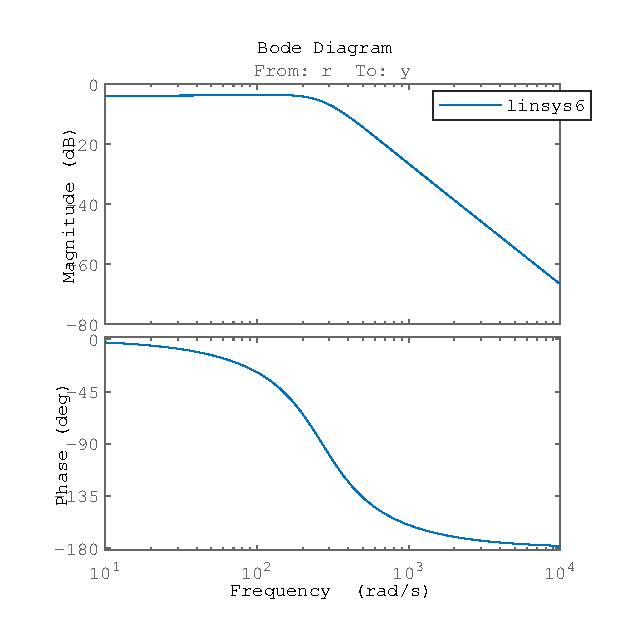
\includegraphics{images/Lab_2_Bode.eps}%
  }\hfill\\
  \subfloat[A much less damped, \(\zeta << 0.707,\) second order system.%
  \label{fig:lab2:bode:b}]{%
    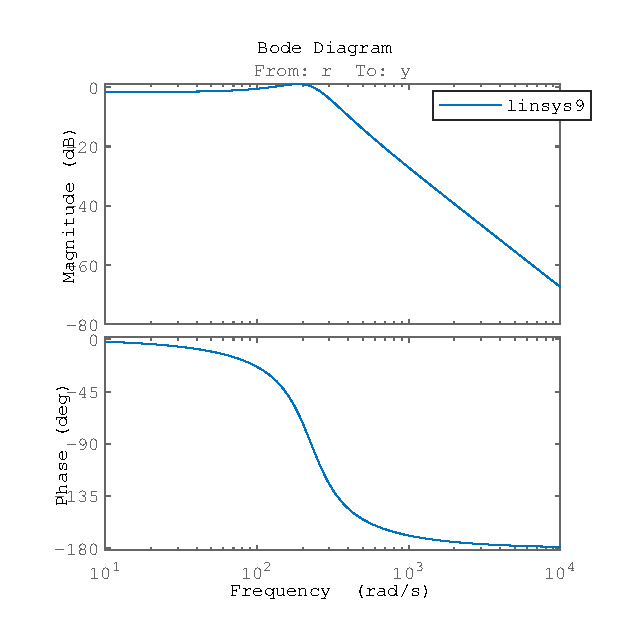
\includegraphics{images/Lab_2_Bode_Peak.eps}%
  }\hfill\\
  \caption[Sample Bode Plots of a Second Order System]{
    Sample Bode plots of a second order system.
  }
  \label{fig:lab2:bode}
\end{figure}
%
\begin{procedure}[label={proc:lab2:p4}]
  \begin{enumerate}[label=(\arabic*)]
    \item{
      \textbf{Put} your system is in the closed-loop configuration as depicted
      in Figure~\ref{fig:lab2:closing-loop}.
      \textbf{Ensure} the gain \(K_p\) is set to \(1.\)
    }
    \item{
      \textbf{Acquire} a Bode plot. \emph{Did you know you can overlay
      this Bode plot on top of the Bode plot of Procedure~\ref{proc:lab2:p3}?
      To do so, take the Bode plot of the open loop system. Then, change the
      configuration. Finally, instead of pressing ``\texttt{Bode Plot}'' press
      a new button with the title of the plot. In my case it was
      ``\texttt{Bode Plot 1}.'' You will have something replicating that of
      Figure~\ref{fig:lab2:bodeclosed}}
    }
  \end{enumerate}
\end{procedure}
%
\begin{figure}
  \centering
  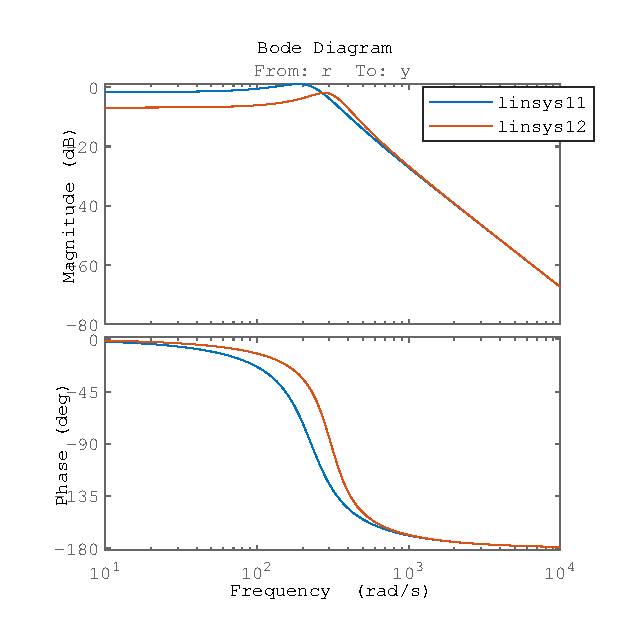
\includegraphics{images/Lab_2_Bode_ClosedLoop.eps}%
  \caption[Sample Overlayed Bode Plots of a Second Order System]{
    Sample overlayed Bode plots of a second order system.
  }
  \label{fig:lab2:bodeclosed}
\end{figure}
%
%
\begin{deliverable}[label={lab2:d3}]
  \textbf{Capture} a Figure depicted the Bode plot found in
  Procedure~\ref{proc:lab2:p4}. \textbf{Include} a data tip measuring
  the bandwidth frequency.
\end{deliverable}
%

\subsection{Disturbance Rejection}
Wow! You are almost done the experimental part of this lab. This section
explores how the closed-loop affects disturbance rejection. Disturbances are
signals that we haven't modelled \emph{or} cannot be modelled and therefore
cannot account for. Naturally, large enough disturbances affect our ability to
control systems. The beauty of control is that we can design systems that
mitigate disturbances we do not explicitly model or know about! Here we will
find that our system can mitigate some types of disturbance signals, but not
all.

\begin{procedure}[label={proc:lab2:p5}]
  For this procedure, you will change the input signal. You will remove the
  ``\texttt{Input Perturbation}'' annotation from the reference \(r\) and
  place it on the disturbance \(d.\)

  \begin{enumerate}[label=(\arabic*)]
    \item{
      \textbf{Ensure} the system is in the closed-loop configuration
      depicted in Figure~\ref{fig:lab2:closing-loop}. \textbf{Set} the gain
      \(K_p\) to \(1.\)
    }
    \item{
      \textbf{Remove} the ``\texttt{Input Perturbation}'' annotation from
      the reference signal. This amounts to repeating the process described
      in Appendix~\ref{App:Simulink:ModelLinearizer:2}, i.e. right click the
      signal wire \(r\) and press
      \texttt{Linear Analysis Points/Input Perturbation}.
    }
    \item{
      \textbf{Add} the ``\texttt{Input Perturbation}'' annotation to the
      the disturbance signal \(d.\)
    }
    \item{
      \textbf{Open} the Model Linearizer App and \textbf{acquire} a Bode
      plot. \emph{Expect the Bode plot to look substantially different than
      your previous Bode plots.}
    }
  \end{enumerate}
\end{procedure}
%
\begin{deliverable}[label={lab2:d4}]
  \textbf{Include} the Bode plot you generated in Procedure~\ref{proc:lab2:p5}
  in you report.
\end{deliverable}

\section{Report Deliverable}
Good job! You made it through Lab~\ref{Lab:2}.
You are required to submit a report
that verifies you completed Lab~\ref{Lab:2} and that you understand the
procedures you performed. In addition to including
\begin{itemize}
  \item{Deliverable~\ref{lab2:d1},}
  \item{Deliverable~\ref{lab2:d2},}
  \item{Deliverable~\ref{lab2:d3a},}
  \item{Deliverable~\ref{lab2:d3} and }
  \item{Deliverable~\ref{lab2:d4}}
\end{itemize}
in your report,
you are required to answer the questions of the following deliverable.
Make sure to leverage your other deliverables in your answers!
\begin{deliverable}[label={lab2:report}]
  \begin{enumerate}[label={(\arabic*)}]
    \item{
      Using the characteristics collected in Step~\ref{proc:lab2:p1:4} of
      Procedure~\ref{proc:lab2:p1}, \textbf{determine} the parameters
      \(\hat{K},\) \(\omega_n\) and \(\zeta\) that describe your plant \(P(s)\)
      in the standard second order form
      \[
        P(s) = \frac{\hat{K} \omega_n^2}{s^2 + 2 \zeta \omega_n s + \omega_n^2}
        .
      \]
      \emph{Hint: What are the formulas that connect the above parameters
      (damping ratio, gain, natural frequency) to the rise time, settling time
      and other parameters?}
      \label{lab2:report:q1}
    }
    \item{
      \textbf{Identify} one another way you could compute \(\omega_n\)
      experimentally given the data you've collected already.
      \label{lab2:report:q2}
    }
    \item{
      For the closed-loop diagram of Figure~\ref{fig:lab2:closing-loop},
      \textbf{compute} the transfer function from \(r\) to \(y.\)
      Then \textbf{compute} the damping ratio and natural frequency of the
      resulting second-order system.
      \label{lab2:report:q3}
    }
    \item{
      Given the open-loop damping ratio and natural frequency found in
      \ref{lab2:report:q1} and closed-loop damping ratio and natural
      frequency found in~\ref{lab2:report:q3},
      \textbf{discuss} how closing the loop
      affects the damping ratio and natural frequency of a second order system.
      \label{lab2:report:q4}
    }
    \item{
      Using Table~\ref{tab:lab2:p2}, \textbf{discuss} how changing the
      gain \(K_p\) affects the various characteristics of the second order
      system. In effect, \textbf{discuss} the benefits and limitations of a
      proportional error feedback control system when applied to a second
      order system. \emph{\textbf{Ensure} you discuss every characteristic
      you've collected; if there is no trend, say so.}
      \label{lab2:report:q5}
    }
    \item{
      Using the bandwidth frequencies found in Procedures~\ref{proc:lab2:p3}
      and~\ref{proc:lab2:p4}, \textbf{discuss} how closing the loop
      changes the bandwidth frequency.
      \label{lab2:report:q6}
    }
    \item{
      \textbf{Why} is it desireable to be able to change the bandwidth
      of a system?
      \label{lab2:report:q7}
    }
    \item{
      Leveraging Deliverable~\ref{lab2:d4}, \textbf{discuss} how well the
      closed loop rejects disturbance signals. \emph{Hint: The Bode plot
      depicts the steady-state gain and phase shift of the output relative
      to the input when the system is hit with an input signal of a given
      frequency (x-axis). In this Bode plot, the input was the disturbance.}
      \label{lab2:report:q8}
    }
    \item{
      For the open-loop configuration, \textbf{derive} the transfer function
      from the disturbance signal \(d\) to the output \(y.\)
      \textbf{Compare} the disturbance rejection properties between the
      open-loop and closed-loop system.
      \label{lab2:report:q9}
    }
    \item{
      \textbf{Derive} the closed-loop transfer function from the
      disturbance \(d\) to the output \(y.\) How do the disturbance rejection
      properties change as you increase \(K_p\)? Do they improve or degrade?
      If so, for what frequencies?
      \label{lab2:report:q10}
    }
  \end{enumerate}
\end{deliverable}

\subsection{Grading Scheme}
The grading scheme is shown in Table~\ref{tab:lab2:grading}. The breakdown of
your grade is shown per deliverable except in the case of the lab
questions where it is shown per question.
%
\begin{table}
\centering
\begin{tabular}{c|l|c}
        & Deliverable           & Weight  \\ \hline
        & \ref{lab2:d1}         & 2       \\ \hline
        & \ref{lab2:d2}         & 2       \\ \hline
        & \ref{lab2:d3a}        & 2       \\ \hline
        & \ref{lab2:d3}         & 2       \\ \hline
        & \ref{lab2:d4}         & 2       \\ \hhline{=|=|=}
Lab Subtotal&                       & 10      \\ \hhline{=|=|=}
        & \ref{lab2:report}~\ref{lab2:report:q1}  & 3       \\ \hline
        & \ref{lab2:report}~\ref{lab2:report:q2}  & 1       \\ \hline
        & \ref{lab2:report}~\ref{lab2:report:q3}  & 3       \\ \hline
        & \ref{lab2:report}~\ref{lab2:report:q4}  & 2       \\ \hline
        & \ref{lab2:report}~\ref{lab2:report:q5}  & 5      \\ \hline
        & \ref{lab2:report}~\ref{lab2:report:q6}  & 1       \\ \hline
        & \ref{lab2:report}~\ref{lab2:report:q7}  & 1       \\ \hline
        & \ref{lab2:report}~\ref{lab2:report:q8}  & 10      \\ \hline
        & \ref{lab2:report}~\ref{lab2:report:q9}  & 2       \\ \hline
        & \ref{lab2:report}~\ref{lab2:report:q10} & 5       \\ \hhline{=|=|=}
Report Subtotal&  & 32 \\ \hhline{=|=|=}
  Total &                       & 42
\end{tabular}
\caption[Grading Scheme for Lab 2]{Grading scheme for Lab 2.}
\label{tab:lab2:grading}
\end{table}
%
